%&LaTeX

\section{The Matlab Lab, or How to Not Teach a Programming Language}

Labs in this class will make liberal use of the Matlab numerical
programming environment. Because this class assumes that you are an
experienced computer science student, you are expected to be able to
learn how to use computer tools, and how to program in new programming
languages, pretty much on your own. So, the first thing you should do
is check out the Matlab documentation built into the Matlab help
system, or online at
\url{http://www.mathworks.com/help/matlab/index.html}. Of course, you
can always search online for Matlab tutorials and the like. We'll
include a very brief overview of Matlab below, and then more detailed
information about the code developed specifically for this class that
you will be using.

\subsection{Matlab in a (Very Small) Nutshell}
\label{sc:basic-matlab}

The Matlab GUI environment is very similar to IDEs that you are
already familiar with. As you might expect, there are some
idiosyncrasies here and there, but nothing terribly unexpected. The
major areas of difference are tools and panes that have to do with
viewing variables (something in other IDEs that you'd only see when
debugging a program), the command pane, and figure windows that open
to display graphs. The first two of these differences have to do with
the fact that Matlab is an interpreted language/programming
environment. You primary area of interaction with the Matlab
interpreter will be through the command window, with variable
information panes providing views of variables and their contents
related to your interaction. It's interesting to note that, if you
want, you can run Matlab without the GUI, providing just a command
line interface.

Interpreted languages have their advantages and disadvantages.  One
advantage is that anything you can use as a line of code in a program
you can use immediately as a command on the command line. This lets
you test code interactively and then copy it into the script or
function you're writing. Like any IDE, Matlab includes an editor with
syntax highlighting and debugger integration.

The disadvantage is the interpreted programs are slower. In Matlab, we
get around this by using built-in functions that operate on entire
vectors or arrays as single data objects. The core loops of the
built-in functions are compiled for speed. If you make good use of
those functions, Matlab code can often be as fast as completely
compiled code.

Here are some things to try:
\begin{enumerate}
\item Immediate calculations and variables:
\begin{lstlisting}[style=Matlab-editor,basicstyle=\mlttfamily\small]
radius = 5    % Comments start with "%"
circumference = 2 * pi * radius
area = pi * radius^2
\end{lstlisting}
\item Complex numbers:
\begin{lstlisting}[style=Matlab-editor,basicstyle=\mlttfamily\small]
sqrt(-1)
x = 7 + 14j
conj(x)       % complex conjugate
abs(x)        % magnitude (e.g., for polar representation)
angle(x)      % and angle for polar rep
real(x)
imag(x)
\end{lstlisting}

\item Complex exponentials:
\begin{lstlisting}[style=Matlab-editor,basicstyle=\mlttfamily\small]
exp(j * pi)
exp(j * pi/2)
exp(j * pi/4)
\end{lstlisting}

\item Vectors:
\begin{lstlisting}[style=Matlab-editor,basicstyle=\mlttfamily\small]
v1 = [0 1 2 3]    % Four elements
v2 = [0 : 2 : 10] % like a loop (start value : increment : end value)
v3 = pi * [-0.5 -0.25 0 0.25 0.5] % All operations are vectorized
exp(j * v3)
mistake = v1 * v1     % a mistake; vector mult doesn't work this way
dotproduct = v1 * v1' % transposing will work, if you want to do this
arrayprod = v1 .* v1  % element-by-element ops include: .+, .-, .*, ./
\end{lstlisting}

\item Simple plots (note that ``;'' suppresses outputting results to
  the command window --- useful if that would generate massive amounts
  of text, or just if you want things neat):
\label{it:simple-plots}
\begin{lstlisting}[style=Matlab-editor,basicstyle=\mlttfamily\small]
t = [0 : 0.01 : 2*pi];
x = sin(t);
plot(t, x);       % default plots points connected by lines in blue
plot(t, x, 'r');  % change the line color
plot(t, x, 'r.'); % change the plot style; zoom in to see individual points
xlabel('t, ms');  % X axis label (all of your plots should have this)
ylabel('Mag');    % Y axis label (all of your plots should have this)
title('Triangle');% Graph title (all of your plots should have this)
\end{lstlisting}

\end{enumerate}

If you take a sequence of commands and save them in a file with an
extension of \texttt{.m}, the result is a \emph{script}. Assuming that the
script is saved in a directory in the MATLAB search path, you can then
execute the script by just typing its name (without the \texttt{.m}),
just as if it were a command. If you want your code to take
parameters, return a return value, and have local variables, start
your code with a line like:
\begin{lstlisting}[style=Matlab-editor,basicstyle=\mlttfamily\small]
function retval = funcname(parm1, parm2)
\end{lstlisting}

Your code is now a function. MATLAB functions can take variable
numbers of arguments and even return variable numbers of return
values, but that's getting beyond what we need right now.

\paragraph{Step 1.1} It's easy to create, concatenate, extract, and modify
vectors or parts of vectors. Execute the following lines of Matlab
code and explain what each echoes out: 
\begin{lstlisting}[style=Matlab-editor,basicstyle=\mlttfamily\small]
a = ones(1,3)
b = zeros(1,5)
x = [b, a, [1:2:12]]
x(7:end)
length(x)
x(1:2:12)
\end{lstlisting}

Also, explain the difference between the square bracket notation
\verb|[1:2:12]| and the parenthetical notation \verb|(1:2:12)|.

\paragraph{Step 1.2} Consider the result of the following assignment:
\begin{lstlisting}[style=Matlab-editor,basicstyle=\mlttfamily\small]
x(7:11) = pi*(1:5)
\end{lstlisting}

Write a \emph{single} statement that will replace the odd-indexed
elements of \texttt{x} with the constant -10 (i.e., \texttt{x(1)},
\texttt{x(3)}, etc).


\paragraph{Step 1.3} One of the side benefits of learning Matlab is
that it trains you to think in terms of parallel operations --- an
increasingly important skill in a profession becoming dominated by
multi-core, GPU, and distributed computing. That doesn't mean you
can't write loops in Matlab; it's just that your code will be more
concise and efficient if you can avoid that. The efficiency arises
from the fact that the vectorized Matlab commands are mostly compiled;
while the loops you write are interpreted. Consider the following loop:
\begin{lstlisting}[style=Matlab-editor,basicstyle=\mlttfamily\small]
for k=0:7,
   x(k+1) = cos(k*pi/4);
end
x
\end{lstlisting}

Why is \verb|x| indexed by \verb|k+1| rather than \verb|k|? What
happens to the length of \verb|x| for each iteration of the loop?
Rewrite this computation without using the loop (as in list
item~\ref{it:simple-plots}). Besides the increase in efficiency from
avoiding an interpreted loop, what other major efficiency results from
this change?

\paragraph{Step 1.4} Consider the following code that plots a
sinusoid:
\begin{lstlisting}[style=Matlab-editor,basicstyle=\mlttfamily\small]
t = [0 : 0.01 : 1]; % time in seconds
f = 5;              % freq in Hertz
x = sin(2*pi*f*t);
plot(t, x);
xlabel('Time (sec)');
\end{lstlisting}

Use the MATLAB editor to create a script file called
\texttt{firstsin.m}, verify that you've saved it in a directory in the
MATLAB path (or add that directory to the path), and test its
execution by typing \texttt{firstsin} at the MATLAB command
prompt. Note that you can also do:
\begin{lstlisting}[style=Matlab-editor,basicstyle=\mlttfamily\small]
type firstsin   % prints out contents of the script
which firstsin  % shows directory (useful when your code shadows built-ins)
\end{lstlisting}

If you included documentation for this script (comments at the
beginning), the command \verb|help firstsin| would also produce useful
output.

Add three lines of code to your script, so that it will plot a cosine
using the same axes as the sine (i.e., ``on top of the sine''). Use
the \texttt{hold} function to add a plot of
\begin{lstlisting}[style=Matlab-editor,basicstyle=\mlttfamily\small]
0.75*cos(2*pi*f*t)
\end{lstlisting}
to the plot. So, your final graph will have two functions
plotted. Save the plot using the MATLAB \texttt{print} command as a
PNG file named \texttt{step14.png} by typing:
\begin{lstlisting}[style=Matlab-editor,basicstyle=\mlttfamily\small]
print -dpng step14
\end{lstlisting}

You should include all plots and code snippets in your lab report,
following the instructions in the report rubric.


\paragraph{Step 1.5} You can also use Matlab to generate sounds. A
pure tone is merely a sinusoid, which you already know how to
generate. Let's generate one with a frequency of 3 kHz and a duration
of 1 second:
\begin{lstlisting}[style=Matlab-editor,basicstyle=\mlttfamily\small]
T = 1.0;
f = 3000;
fs = 8000;
t = [0 : (1/fs) : T];
x = sin(2*pi*f*t);
soundsc(x, fs)
\end{lstlisting}

The vector of numbers \texttt{x} are converted into a sound waveform
at a certain rate, \verb|fs|, called the \emph{sampling rate} (we will
learn a lot more about this in this class). In this case, the sampling
rate was set to 8000 samples/second. What is the length of
the vector \texttt{x}?

\paragraph{Step 1.6} Write a new function that performs the same task
as the following function without using any loops. Use the idea in
step~1.3 and also consult the section on the \verb|find| function,
relational operators, and vector logicals in the MATLAB documentation.
\begin{lstlisting}[style=Matlab-editor,basicstyle=\mlttfamily\small]
function B = denegify(A)
% DENEGIFY Replace negative elements of matrix with zeros
% Usage:
%    B = denegify(A)
%
[W,H] = size(A);
for i=1:W
   for j=1:H
      if A(i,j) < 0
         B(i,j) = 0;
      else
         B(i,j) = A(i,j);
      end
   end
end
\end{lstlisting}



\subsection{Trigonometric Functions and Complex Mathematics in Matlab}


\paragraph{Step 2.1} In this step, you are asked to complete a Matlab
function to synthesize a waveform in the form of:
\begin{equation*}
x(t) = \sum_{k=1}^N a_k\cos(2\pi f t + \phi_k)
\end{equation*}
This is a sum of cosines, all at the same frequency but with different
phases and amplitudes.  Use the following function prototype to start you off:
\begin{lstlisting}[style=Matlab-editor,basicstyle=\mlttfamily\small]
   function x = sumcos(f, phi, a, fs, dur)
   % SUMCOS Synthesize a sum of cosine waves
   % Usage:
   %    x = sumcos(f, phi, a, fs, dur)
   %        Returns sum of cosines at a single frequency f, sampling
   %        rate fs, and duration dur, each with a phase phi and
   %        amplitude a.
   %    f = frequency (scalar)
   %    phi = vector of phases
   %    a = vector of amplitudes
   %    fs = the sampling rate in Hz (scalar)
   %    dur = total time duration of signal (scalar)
\end{lstlisting}


Include your code in your writeup. Additionally, include a plot of
\texttt{x = sumcos(20, [0 pi/4 pi/2 3*pi/2], [1 2 3 4], 200, 0.25);} versus
time.

Hint: the MATLAB \verb|length| function is useful in determining the
number of elements in a vector; the \verb|size| function returns both
dimensions of a vector or an array.


\paragraph{Step 2.2} Now, let's see how complex exponentials can
simplify things. Re-implement your \texttt{sumcos} function using
complex exponentials. Take advantage of the fact that multiplying a
complex sinusoid $e^{j2\pi f t}$ by the complex amplitude
$a_ie^{j\phi}$ will shift its phase and change its amplitude. Thus,
you should be able to create a \emph{single} complex sinusoid at the
given frequency \texttt{f} and then multiply it by different \texttt{a
  * exp(j * phi)} to get multiple phase shifted cosines. Remember that
we want a real value to plot; the cosine is the real part of a complex
sinusoid. Include your code in your writeup and provide a plot that
demonstrates that this function produces the same result as the
original implementation.


\paragraph{Step 2.3} Generate four sinusoids with the following
amplitudes and phases:
\begin{align}
x_1(t) &= 6 \cos(2\pi(10)t - 0.5\pi) \\
x_2(t) &= 3 \cos(2\pi(10)t + 0.25\pi) \\
x_3(t) &= 2 \cos(2\pi(10)t - 0.3\pi) \\
x_4(t) &= 8 \cos(2\pi(10)t + 0.9\pi) 
\end{align}

\begin{enumerate}\renewcommand{\theenumi}{\alph{enumi}}
\item Make a single plot of all four signals together over a range of
  $t$ that will generate approximately 3 cycles. Make sure the plot
  includes negative time so that the phase at $t = 0$ can be
  measured. In order to get a smooth plot make sure that your have at
  least 20 samples per period of the wave. Include your plot in your
  writeup.

\item Verify that the phase of all four signals is correct at $t = 0$,
  and also verify that each one has the correct maximum amplitude. Use
  \verb|subplot(3,2,i)| to make a six-panel subplot that puts all of
  these plots in the same figure, with space for two additional plots
  at the bottom. Use the \verb|xlabel|, \verb|ylabel|, and
  \verb|title| functions so that the reader can figure out what the
  plots mean; reinforce this with your report's figure caption. (You
  should include the final figure, with all subplots, that results
  from finishing all of the parts of this step.)

\item Create the sum sinusoid,
  $x_5(t)=x_1(t)+x_2(t)+x_3(t)+x_4(t)$. Plot $x_5(t)$ over the same
  range of time as used in the last plot. Include this as the lower
  left panel in the plot by using \verb|subplot(3,2,5)|.

\item Now do some complex arithmetic; create the complex amplitudes
  corresponding to the sinusoids $x_i(t)$: $z_i = A_ie^{j\phi_i}$,
  $i=1,2,3,4,5$. Include a table in your report of the $z_i$ in polar
  and rectangular form, showing $A_i$, $\phi_i$, $\Real\{z_i\}$, and
  $\Imag\{z_i\}$.
\end{enumerate}


\subsection{Representing Analog, Discrete, and Digital Signals}

In our class, we will need to manipulate analog signals (real-valued
signals that are functions of continuous time), discrete signals
(real-valued signals that are functions of discrete time), and digital
signals (discrete-valued signals that are functions of discrete
time). No need to worry about the details or these; that will become
clear later. The trickiest part of this is representing anything other
than digital signals on a digital computer, because you can't. So,
we'll need to employ two key elements of software design: information
hiding and make-believe.

\begin{figure}
\begin{center}
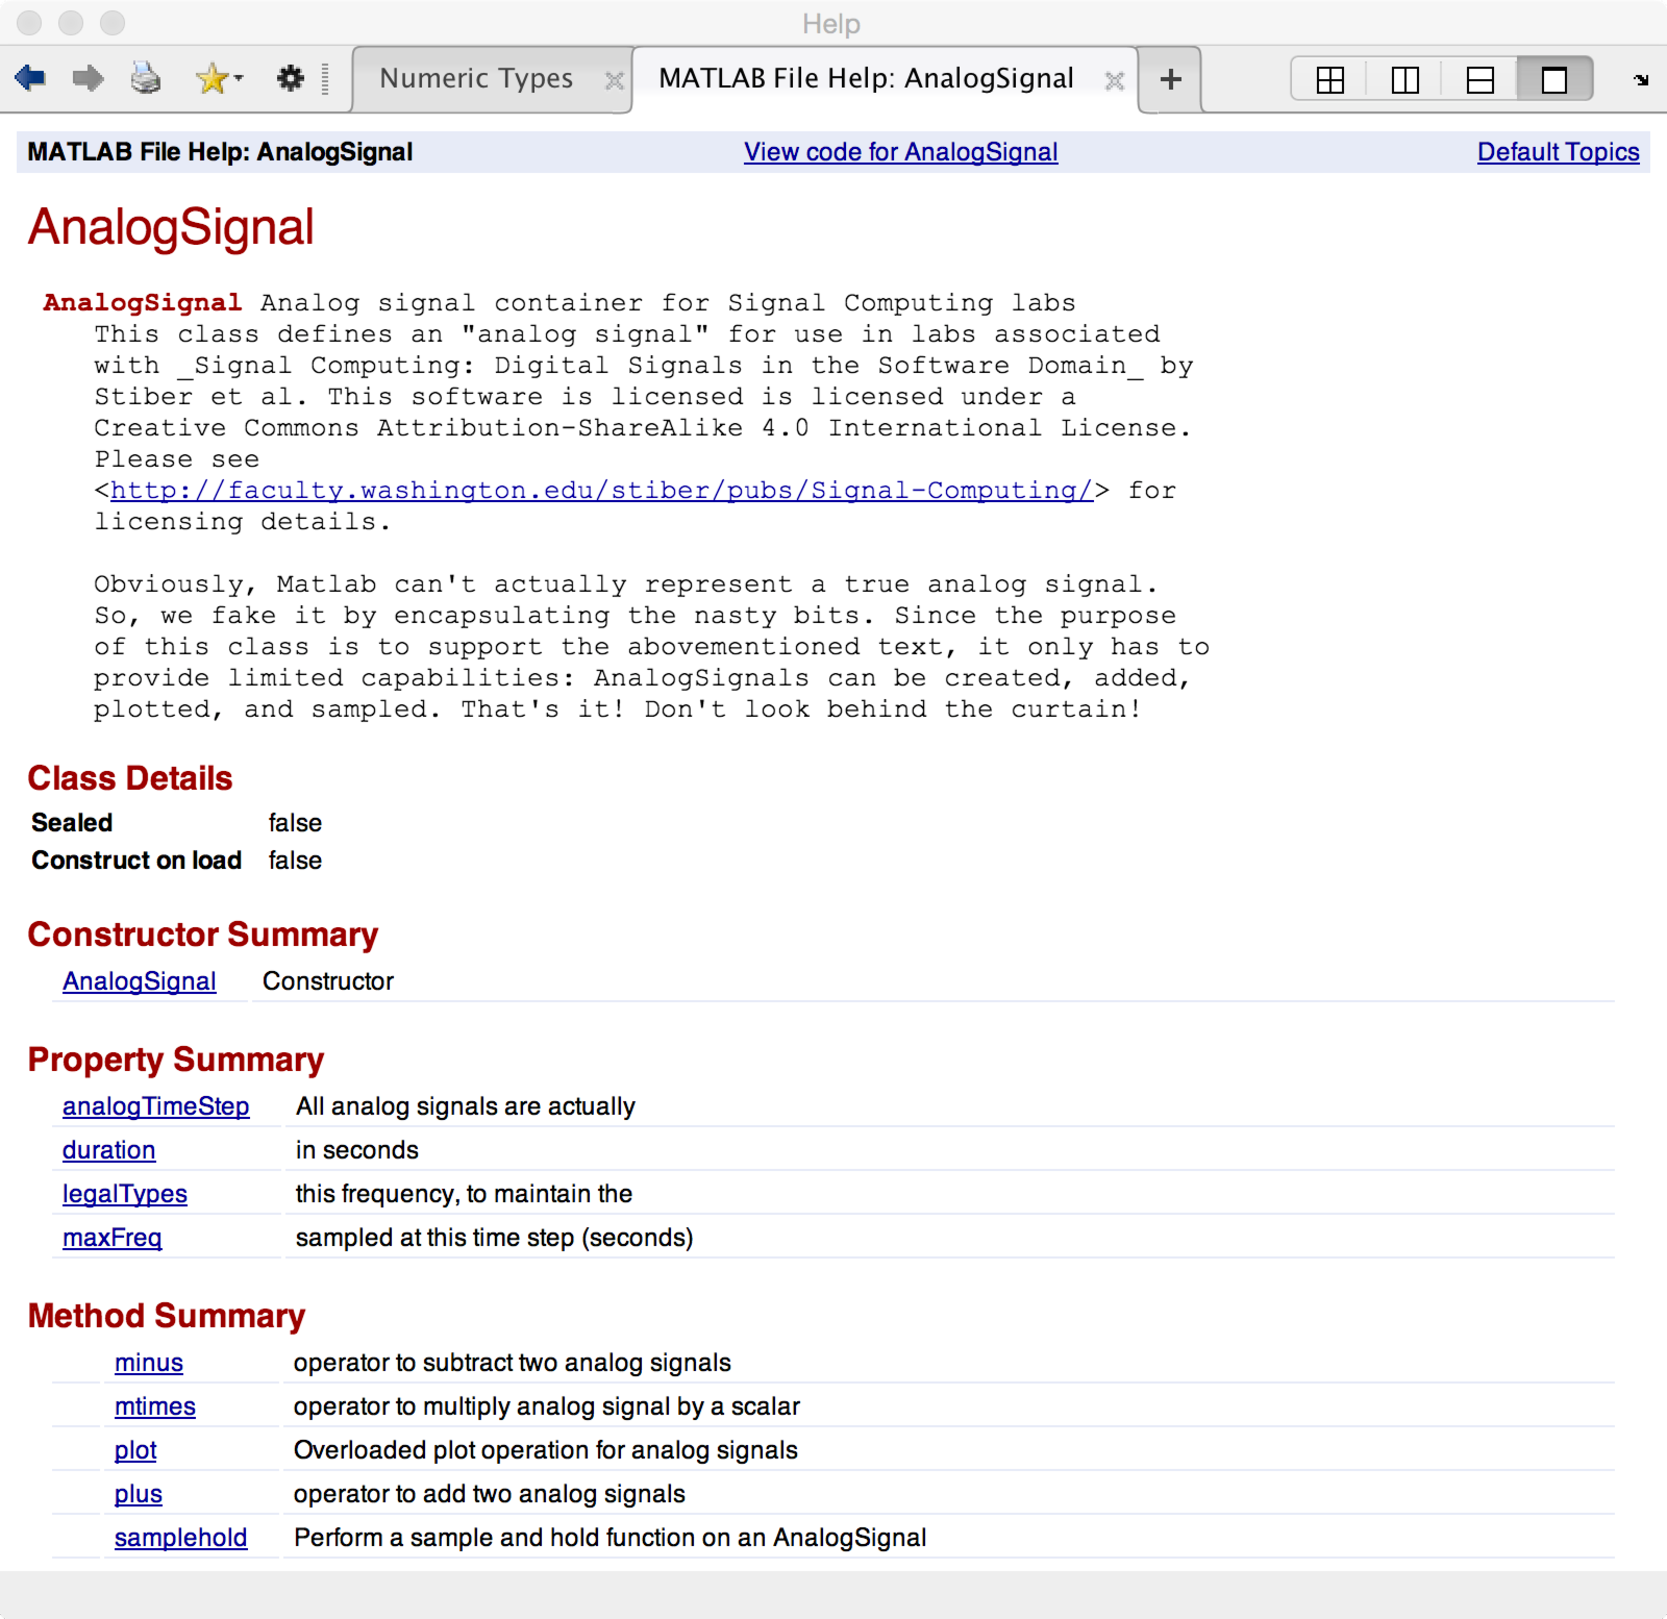
\includegraphics[width=0.75\textwidth]{lab1/AnalogSignal-help}
\end{center}
\caption{Example help screen for the \texttt{AnalogSignal}
  class. This example may be out-of-date; use the Matlab
  \texttt{doc AnalogSignal} command to get current
  documentation.\label{fg:analogsignal-help}}
\end{figure}

Information hiding is used in our implementation of analog signals. We
make use of the object-oriented programming aspects of Matlab to
create an \texttt{AnalogSignal} class. If you look up the
documentation for \texttt{AnalogSignal} (using
\verb|doc AnalogSignal|), you'll see something like
figure~\ref{fg:analogsignal-help}. The key operations on these analog
signals are:
\begin{itemize}
\item Creating an analog signal (ex: \texttt{a =
    AnalogSignal('sawtooth', 2.0, 1.0, 10.0)}).
\item Scaling an analog signal (ex: \texttt{b = a * 5})
\item Adding two analog signals (ex: \texttt{c = a + b})
\item Subtracting two analog signals (ex: \texttt{d = c - a})
\item Plotting an analog signal (ex: \texttt{plot(d)})
\item Sampling an analog signal (ex: \texttt{x = d.samplehold(0.1)})
\end{itemize}

You will get a lot more experience working with analog signals shortly
in this class, so for the time being just play with this a bit.

